 \begin{figure}[!ht]
	\begin{center}
		\makebox[\textwidth]{
			\centering
			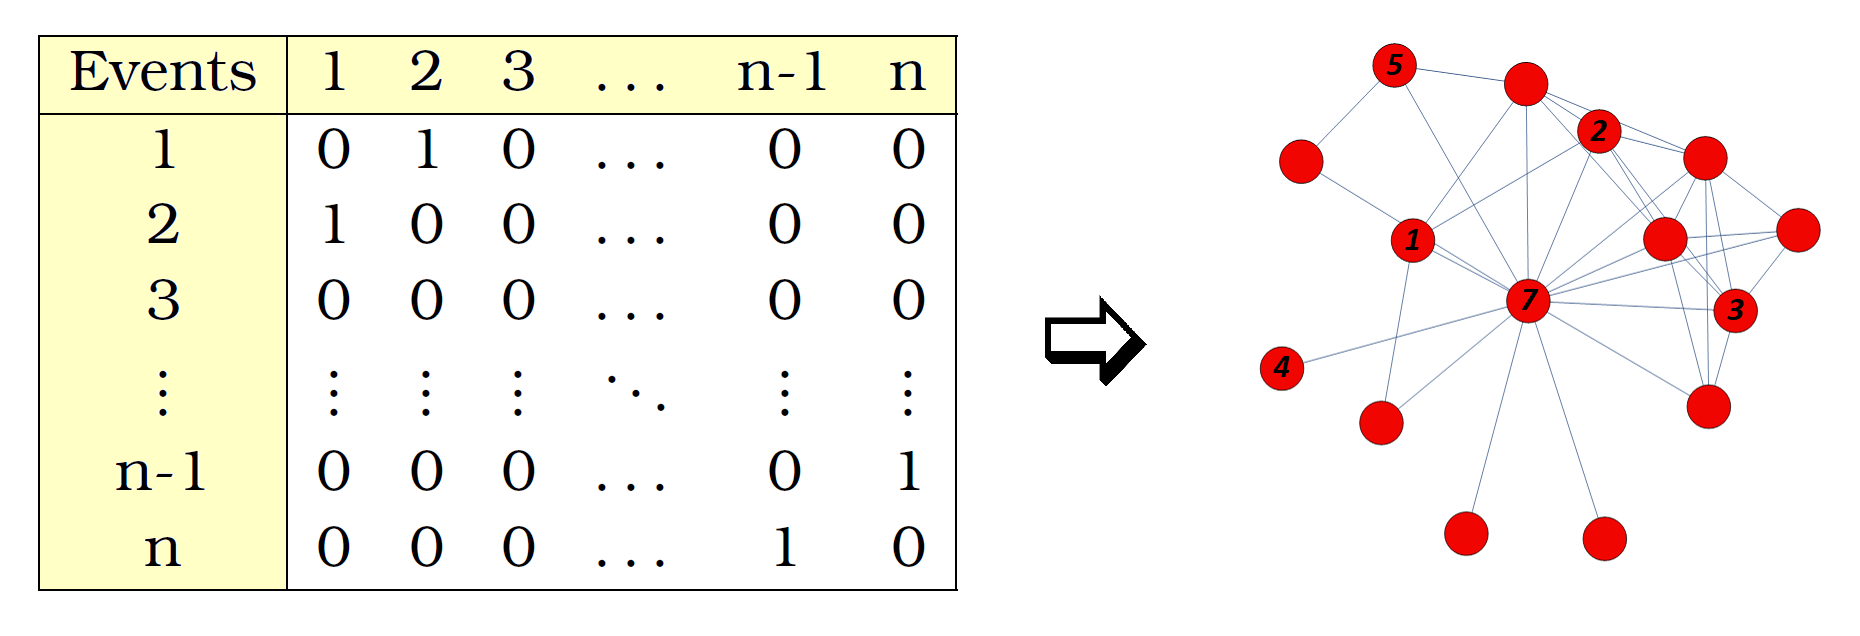
\includegraphics[width=0.7\linewidth]{../images/methodology-association-networks-adjacency_graph.png}}
		\caption{An Arbitrary Representation for Adjacency Matrix and its Graph.}
		\label{figure-adjacency_graph}
	\end{center}
\end{figure}

%\begin{table}[]
%	\begin{tabular}{|c|cccccc|}
%		\hline
%		Events & 1   & 2   & 3   & \dots & n-1 & n   \\ \hline
%		1      & 0   & 1   & 0   & \dots & 0   & 0   \\
%		2      & 1   & 0   & 0   & \dots & 0   & 0   \\
%		3      & 0   & 0   & 0   & \dots & 0   & 0   \\
%		\vdots & \vdots & \vdots & \vdots & \ddots & \vdots & \vdots \\
%		n-1    & 0   & 0   & 0   & \dots & 0   & 1   \\
%		n      & 0   & 0   & 0   & \dots & 1   & 0   \\ \hline
%	\end{tabular}
%\end{table}